% Fragmento para incorporação ao relatório principal do projeto PRO3474.
% Pacotes pressupostos no preâmbulo do documento que incorporar este arquivo:
%   inputenc (utf8), fontenc (T1), graphicx, longtable, booktabs, array, geometry (margens compatíveis com tabelas largas).
% Figuras referenciadas em figures/ (caminho relativo a este arquivo).

\section{Análise dos clientes}

\subsection{Fontes e abordagem metodológica}

Esta análise teve como objetivo responder a três perguntas: quem são os clientes observados na experiência de compra em loja física da Riachuelo, como esses clientes podem ser agrupados a partir de comportamentos e contextos relevantes para a jornada de compra, e o que esses clientes procuram, valorizam ou enfrentam ao longo dessa jornada. A tradução desses achados em necessidades, desejos e demandas preliminares, apresentada na Seção~\ref{sec:ndd}, foi tratada como etapa posterior, e não como ponto de partida da leitura dos dados.

Foram utilizadas duas fontes primárias, complementadas por dois documentos de apoio. A primeira fonte foi um survey estruturado, intitulado \emph{Pesquisa de Experiência de Compra em Loja}, aplicado junto a consumidores e exportado em 142 respostas válidas. O instrumento teve seis páginas e 25 campos, combinando itens de escala Likert de 1 a 5 com itens de frequência (de \emph{Nunca} a \emph{Sempre}), organizados em cinco blocos temáticos: disponibilidade e facilidade de encontrar produtos; atendimento e autonomia; filas, pagamento e tempo na loja; confiança em tecnologia e canais digitais; segurança e confiança na compra. O item central para a hipótese de solução em estudo foi \emph{Confiaria em um processo de compra que não exigisse checagem manual na saída, desde que o pagamento já estivesse confirmado}. Um problema no registro do formulário fez com que os 142 carimbos de data e hora do arquivo exportado aparecessem concentrados num intervalo de poucos minutos, embora a coleta tenha ocorrido ao longo de uma semana. Essa falha não compromete o conteúdo das respostas e não motivou a exclusão de nenhum registro: todas as 142 respostas foram usadas na análise.

A segunda fonte foi um conjunto de onze entrevistas individuais semiestruturadas, conduzidas com um roteiro dividido em blocos temáticos: abertura e contexto, reconstrução de uma jornada de compra recente, busca e disponibilidade de produto, autonomia e atendimento do vendedor, fila e pagamento, confiança e segurança, necessidades não previstas, e, apenas ao final, exploração da hipótese de solução em estudo. O roteiro foi desenhado para que o entrevistado descrevesse experiências concretas em vez de opiniões abstratas, e para que a etiqueta de segurança inteligente só fosse mencionada depois de o entrevistado relatar livremente sua jornada de compra, suas fontes de fricção e suas preferências de atendimento. Essa ordem foi respeitada na leitura dos resultados: os achados sobre caracterização e agrupamento de clientes, apresentados nas Seções~\ref{sec:caracterizacao} e \ref{sec:clusters}, não partem da solução em estudo.

Como documentos de apoio, foi consultado o roteiro de entrevista na íntegra, para confirmar a intenção de cada bloco de perguntas, e uma nota anterior sobre o desenho do survey, que descreve os cinco perfis comportamentais usados para orientar a construção do instrumento e a composição da amostra de entrevistados: autônomo digital, pragmático equilibrado, dependente de atendimento, cético tradicional e frustrado com disponibilidade. Esses cinco perfis foram tratados nesta análise como hipóteses de partida, não como resultado. Ao longo do texto, a análise mostra em que medida esses perfis se confirmam nos dados, onde se fundem, e onde um comportamento relatado não se encaixa bem em nenhum deles.

A abordagem analítica partiu dos dados brutos do survey, sem carregar os rótulos de perfil originais em nenhuma etapa de agrupamento. As perguntas foram recodificadas para escalas numéricas de 0 a 100 e combinadas em dimensões comportamentais (detalhadas na Seção~\ref{sec:quantitativa}). Sobre essas dimensões foram testados agrupamentos por \emph{k-means} e por clusterização hierárquica (Ward), comparando diferentes números de grupos pelo coeficiente de silhueta. As onze entrevistas foram lidas na íntegra, tema a tema, e as falas mais reveladoras foram organizadas por padrão de comportamento. Os rótulos de perfil originais só voltam a aparecer na Seção~\ref{sec:integracao}, para comparar o resultado emergente com o ponto de partida do projeto.

Uma limitação transversal a toda a análise deve ser registrada desde já. A amostra de 142 respostas de survey e 11 entrevistas é pequena, e os materiais disponíveis não documentam como os respondentes e entrevistados foram recrutados ou selecionados. Isso impede avaliar se a amostra é razoavelmente aleatória, concentrada por conveniência, ou enviesada por algum canal específico de recrutamento. As proporções, correlações e agrupamentos discutidos neste documento devem ser lidos como padrões observados nesta amostra específica, e não como estimativas validadas para o conjunto de clientes da Riachuelo. Onde a evidência permitir apenas uma leitura qualitativa, isso é indicado explicitamente no texto.

\subsection{Caracterização dos clientes}
\label{sec:caracterizacao}

\subsubsection{Perfil sociodemográfico e de frequência de compra}

A amostra do survey concentrou-se na faixa de 25 a 34 anos (32\% dos respondentes), seguida por 35 a 44 e 45 a 54 anos (17\% cada). O gênero predominante foi feminino (53\%), seguido de masculino (42\%), com uma pequena parcela não binária ou que preferiu não informar. A frequência de compra em loja física dividiu-se entre \emph{mensalmente} (44\%) e \emph{algumas vezes ao ano} (43\%), com uma minoria comprando mais de uma vez por mês (13\%). A amostra distribuiu-se por vinte shoppings e regiões diferentes de São Paulo e Campinas, sem concentração forte em nenhum, o que limita qualquer leitura por loja específica (Figura~\ref{fig:perfil_demografico}).

\begin{figure}[htbp]
    \centering
    \textbf{Perfil demográfico}
    \caption{Perfil demográfico (faixa etária) e frequência de compra em loja física da amostra do survey (n = 142).}
    \label{fig:perfil_demografico}
\end{figure}

As onze entrevistas cobriram uma faixa etária mais ampla no relato, de jovens como Thiago e Luana a aposentados como Nivaldo e Robério, e uma variedade de papéis de compra (para si, para o cônjuge, para os filhos, para o próprio negócio) que o survey não capturou diretamente, mas que ajudou a interpretar o que estava por trás das respostas de escala.

Como será mostrado na Seção~\ref{sec:quantitativa}, a idade apresentou associação apenas moderada com o comportamento observado, e outras variáveis demográficas, como gênero e loja frequentada, explicaram uma fração ainda menor da variação entre respondentes. Por esse motivo, esta análise não reduziu a caracterização dos clientes a variáveis sociodemográficas: os comportamentos relatados a seguir mostraram maior poder explicativo.

\subsubsection{Papel da compra: para si e para terceiros}

A maioria dos episódios relatados nas entrevistas envolveu compra para o próprio entrevistado. Uma entrevista, a de Wagner, descreveu uma jornada estruturalmente distinta: comprar roupa para os três filhos, sem eles presentes. Nesse caso, a incerteza não recaiu sobre o que comprar (cor, modelo), e sim sobre uma variável que o comprador não podia verificar sozinho, o corpo de outra pessoa: \emph{"Foi bem tentando adivinhar, sinceramente. Eu tirei uma foto da etiqueta de uma calça dele em casa antes de sair, mas mesmo assim eu fico inseguro porque cada marca tem um tamanho diferente"} (Entrevista 10). O survey não tem nenhum item que identifique para quem a peça está sendo comprada, o que impede estimar, a partir dos dados quantitativos, que fração da amostra vive uma situação semelhante à de Wagner.

\subsubsection{Companhia na compra e contexto emocional}

As entrevistas revelaram uma variação relevante no papel da companhia durante a compra, distinta simplesmente de ir sozinho ou acompanhado. Para Marisa e Robério, ir acompanhado (da filha, da esposa) funcionou como um recurso de apoio à decisão: \emph{"Ela que me ajuda a escolher, porque sozinho eu me perco um pouco"} (Entrevista 3). Para Camila, a companhia de uma amiga fez parte do caráter de lazer da visita, sem relação com dependência de decisão: a compra funcionou como \emph{"um passeio"}, não como tarefa. Essa distinção é relevante porque um mesmo comportamento superficial (comprar acompanhado) correspondeu a motivações diferentes: apoio à decisão em um caso, experiência social recreativa em outro. O survey não permite separar essas duas motivações, já que não perguntou sobre companhia na compra.

\subsubsection{Autonomia como preferência variável por etapa da jornada, não como traço fixo}

Um padrão recorrente nas entrevistas foi a coexistência, na mesma pessoa, de preferência por resolver uma etapa da jornada sozinha e de dependência de ajuda em outra etapa, sem que isso fosse relatado como contradição pelo próprio entrevistado. Camila descreveu essa divisão de forma direta: \emph{"A parte de escolher e experimentar, com certeza. Gosto de fazer isso no meu ritmo, sem ninguém em cima"}, e, na mesma entrevista, sobre o que uma vendedora resolve que ela não resolveria sozinha: \emph{"Achar tamanho que sumiu da araque, isso sim eu peço ajuda"} (Entrevista 8). O mesmo padrão apareceu, com variações, em quase todas as entrevistas: a autonomia desejada concentrou-se na escolha e na experimentação, e cedeu lugar à dependência de ajuda especificamente quando o produto procurado não estava visível ou disponível na araque. Esse achado qualitativo sugere que autonomia, tal como o survey a mede (um único conjunto de itens agregados em uma dimensão, ver Seção~\ref{sec:quantitativa}), pode não corresponder a um traço estável do cliente, e sim a uma preferência que varia por etapa da jornada. Essa é uma interpretação construída a partir das entrevistas, não uma medição direta, já que o survey não testou autonomia separadamente por etapa.

\subsubsection{Busca de produto e confiança em canais digitais}

A dificuldade de localizar produtos dentro da loja apareceu com frequência distinta entre entrevistados, mas de forma quase universal em algum grau. Marisa relatou: \emph{"Demais. Principalmente pra mim mesma, que eu uso um tamanho que sempre falta. Isso é bem frequente, viu"} (Entrevista 1). Três entrevistados (Joyce, Felipe e Renata) relataram, de forma independente, ter perdido confiança na informação de estoque exibida por site ou aplicativo depois de uma experiência de divergência entre o que viram online e o que encontraram na loja: \emph{"Porque já aconteceu de eu ver uma coisa disponível no site e chegar lá e não achar, aí acabei desconfiando, sabe. Prefiro ir olhar com meus próprios olho"} (Joyce, Entrevista 2). Esse padrão qualitativo é relevante porque uma parcela da amostra parte de uma credibilidade já corroída em relação a canais digitais de disponibilidade, e não de uma expectativa neutra, o que a leitura puramente quantitativa do item correspondente do survey (Seção~\ref{sec:quantitativa}) não captura sozinha.

\subsubsection{Sensibilidade a fila e a provador}

A definição de problema vigente no projeto trata o intervalo entre decidir comprar e conseguir sair da loja como o núcleo da fricção observada. As entrevistas confirmaram esse intervalo como fonte real de fricção para parte dos entrevistados, mas também apontaram um contraponto que a formulação atual do problema não cobre: para quem valorizou atendimento, a fricção mais citada não foi a fila do caixa, e sim a fila do provador ou a espera por um vendedor disponível. Marisa descreveu o provador como algo recorrente, não excepcional: \emph{"Acho que o provador é uma coisa que pesa bastante, viu. Poucas cabine, fila grande, isso atrapalha demais, principalmente em dia de promoção"} (Entrevista 1). Esse achado qualitativo devolve à definição de problema um contraponto específico de escopo: a fricção entre decidir comprar e sair da loja pode incluir etapas anteriores ao caixa, como prova e disponibilidade de cabine, que a formulação centrada no destravamento pós-pagamento não cobre diretamente.
\subsection{Identificação dos grupos de clientes}
\label{sec:clusters}

\subsubsection{Da hipótese de cinco perfis a uma tipologia de quatro grupos}

O survey foi originalmente desenhado a partir de cinco perfis hipotéticos: consumidoras com menor autonomia e maior insegurança tecnológica, consumidores orientados à eficiência, consumidoras orientadas à experiência e conveniência, pessoas comprando para terceiros (sobretudo filhos), e um grupo residual de respondentes diversos. Esses cinco perfis orientaram o desenho do instrumento e a composição da amostra de entrevistados, e foram tratados nesta análise como hipóteses de partida a verificar, não como categorias obrigatórias de segmentação.

A verificação partiu da estrutura de correlação entre cinco dimensões comportamentais construídas a partir dos itens do survey: autonomia (preferência por resolver e pagar sozinho, com os itens de dependência de vendedor invertidos), confiança em tecnologia, pré-pesquisa digital (consulta a site ou aplicativo antes de ir à loja), sensibilidade à fila, e dor de disponibilidade (dificuldade de encontrar tamanho ou cor, desconhecimento prévio de estoque, saídas sem comprar). A Figura~\ref{fig:correlacao} mostra que quatro dessas cinco dimensões, autonomia, confiança em tecnologia, pré-pesquisa digital e sensibilidade à fila, se correlacionaram fortemente entre si (0,77 a 0,92): nesta amostra, quem se mostrou mais autônomo também confiou mais em tecnologia, pesquisou mais antes de ir à loja e se incomodou mais com fila. A dor de disponibilidade, em contraste, mostrou-se quase independente das outras quatro (correlações entre $-0,22$ e $0,15$).

\begin{figure}[htbp]
    \centering
    \textbf{Correlação}
    \caption{Correlação entre as cinco dimensões comportamentais construídas a partir do survey (n = 142).}
    \label{fig:correlacao}
\end{figure}

Esse é um dado observado, não uma interpretação: as correlações medidas nesta amostra reduzem o espaço de diferenciação real a duas dimensões, e não cinco. A explicação para a alta correlação entre as quatro primeiras dimensões permanece como hipótese em aberto: pode refletir um traço de disposição coerente, no qual pessoas com rotina mais apertada tendem a ser, ao mesmo tempo, mais adeptas de tecnologia, mais autônomas e mais impacientes com fila, ou pode refletir, ao menos em parte, um viés de resposta comum em survey de autorrelato, no qual respondentes tendem a concordar ou discordar de forma consistente ao longo de itens redigidos de forma parecida, independentemente do conteúdo específico de cada um. Os dados atuais não permitem separar as duas explicações. As entrevistas trazem ao menos um contraexemplo direto a uma fusão automática entre autonomia e confiança em tecnologia: Nivaldo descreveu-se como autônomo na escolha do produto, mas desconfiado do pagamento por celular (Entrevista 5), o que reforça que a fusão observada no survey deve ser lida como um padrão desta amostra, não como lei geral de comportamento do consumidor.

A partir dessa constatação, os agrupamentos foram construídos sobre duas dimensões não redundantes: um índice combinado de autonomia, confiança em tecnologia, pré-pesquisa digital e sensibilidade à fila, chamado nesta análise de orientação autonomia-tecnologia-eficiência, e a dor de disponibilidade, mantida separada por ser quase independente da primeira. Foram testados \emph{k-means} e clusterização hierárquica (Ward) para números de grupo entre 2 e 7, comparando o coeficiente de silhueta de cada solução. Os dois métodos convergiram para os mesmos números e tamanhos de grupo. O melhor equilíbrio entre coesão dos grupos e interpretabilidade, sem grupo residual muito pequeno, apareceu em quatro grupos (silhueta de 0,55; uma solução com cinco grupos melhorou marginalmente a silhueta ao custo de isolar um grupo de apenas nove respondentes, tratado como ruído estatístico e não como um quinto agrupamento).

Essa clusterização formal deve ser lida pelo que é: uma técnica exploratória aplicada a 142 respostas de survey, com itens de escala de variação adequada para sustentá-la, e não o critério final e definitivo dos agrupamentos de clientes da Riachuelo. A Seção~\ref{sec:integracao} cruza os quatro grupos identificados com o material qualitativo das entrevistas, e ajusta a interpretação onde a evidência qualitativa exige nuance que a clusterização quantitativa, isoladamente, não captura.

\begin{figure}[htbp]
    \centering
    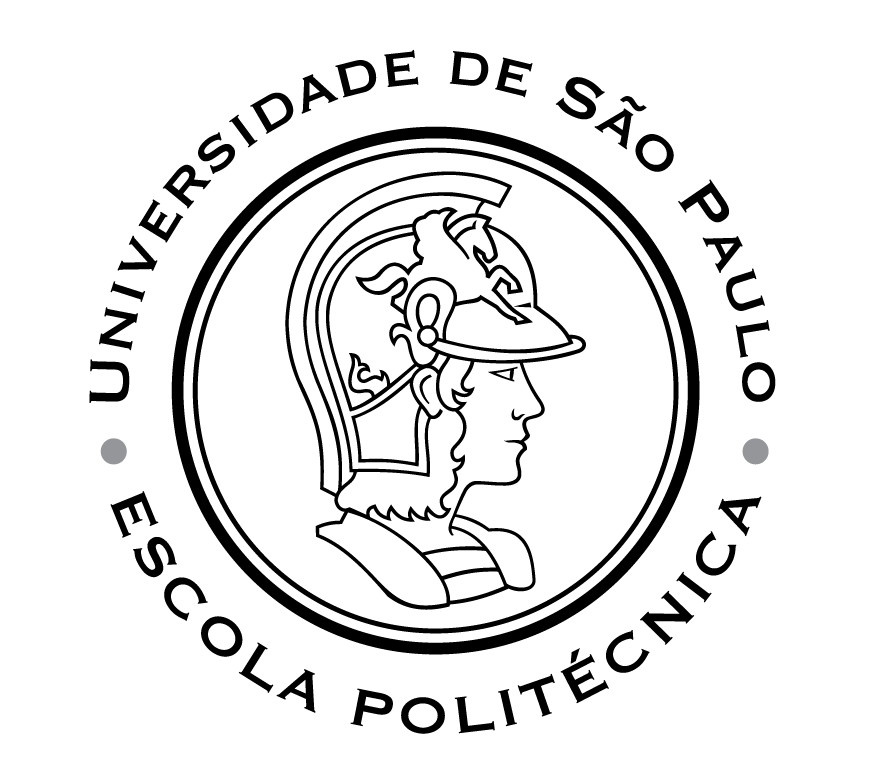
\includegraphics[width=0.8\textwidth]{imagens/Poli.png}
    \caption{Distribuição dos respondentes nos dois eixos usados para a clusterização exploratória: orientação autonomia-tecnologia-eficiência e dor de disponibilidade (n = 142).}
    \label{fig:clusters_scatter}
\end{figure}

\begin{figure}[htbp]
    \centering
    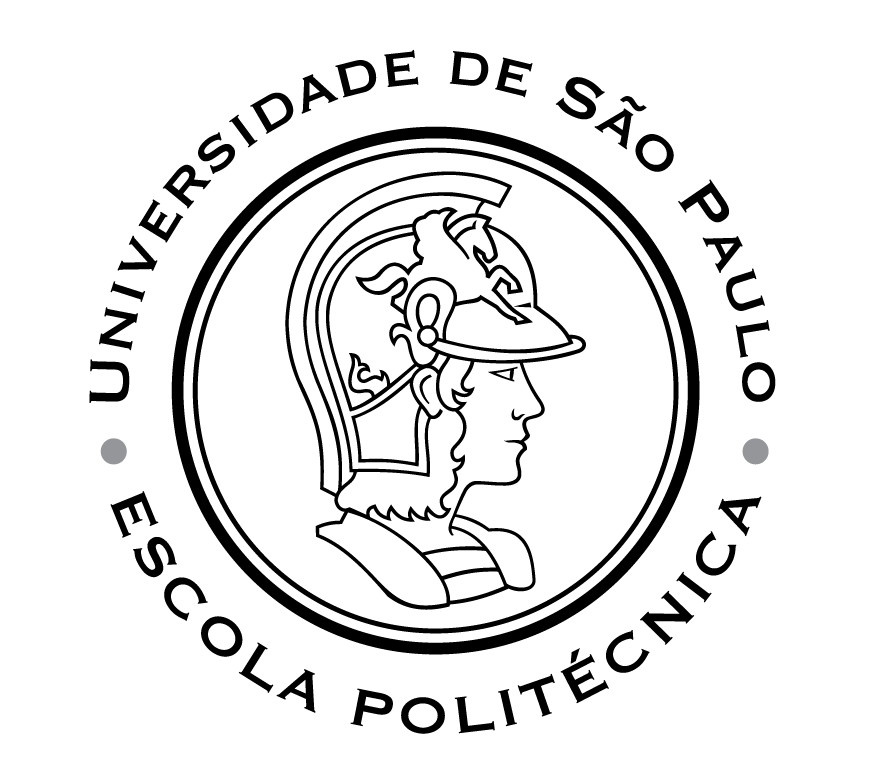
\includegraphics[width=0.8\textwidth]{imagens/Poli.png}
    \caption{Tamanho dos quatro agrupamentos exploratórios identificados (n = 142).}
    \label{fig:tamanho_clusters}
\end{figure}

Os quatro grupos que emergiram não reproduziram exatamente os cinco perfis originais do survey. Três deles tiveram tamanho relativamente próximo a três dos perfis originais, o que sugere que o instrumento os capturou razoavelmente bem. O quarto perfil original, cético tradicional, não apareceu como grupo separado: seus 13 respondentes esperados parecem ter se fundido ao grupo de menor autonomia, junto com o antigo perfil dependente de atendimento (39 mais 13 igual a 52, próximo aos 55 respondentes observados nesse grupo). Esse resultado foi tratado como achado, não como erro de método, e é discutido na Seção~\ref{sec:cluster_aberto} e retomado na síntese (Seção~\ref{sec:sintese}).

As Figuras~\ref{fig:confianca_cluster} e \ref{fig:desistencia_cluster} comparam os quatro grupos nos dois itens mais decisivos da análise: a reação ao conceito de desbloqueio sem checagem manual, e a frequência com que os respondentes já desistiram de uma compra por causa de fila. Ambas mostram um padrão qualitativamente diferente entre grupos, e não apenas de intensidade diferente, o que orientou a construção das fichas de cada cluster a seguir.

\begin{figure}[htbp]
    \centering
    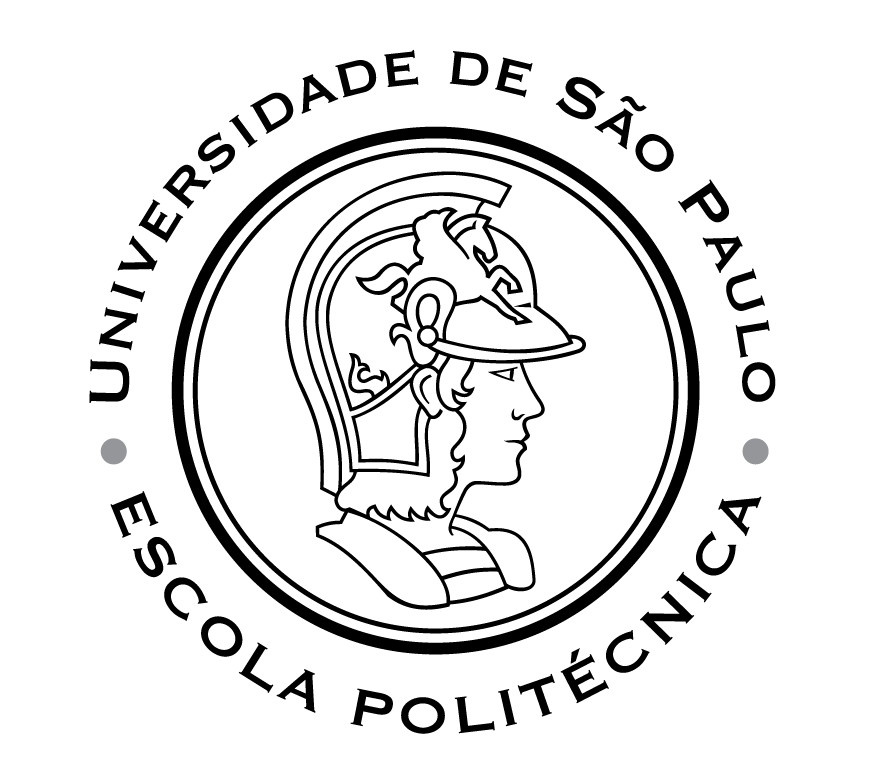
\includegraphics[width=0.8\textwidth]{imagens/Poli.png}
    \caption{Distribuição de respostas ao item de confiança em processo de compra sem checagem manual na saída, por agrupamento (n = 142).}
    \label{fig:confianca_cluster}
\end{figure}

\begin{figure}[htbp]
    \centering
    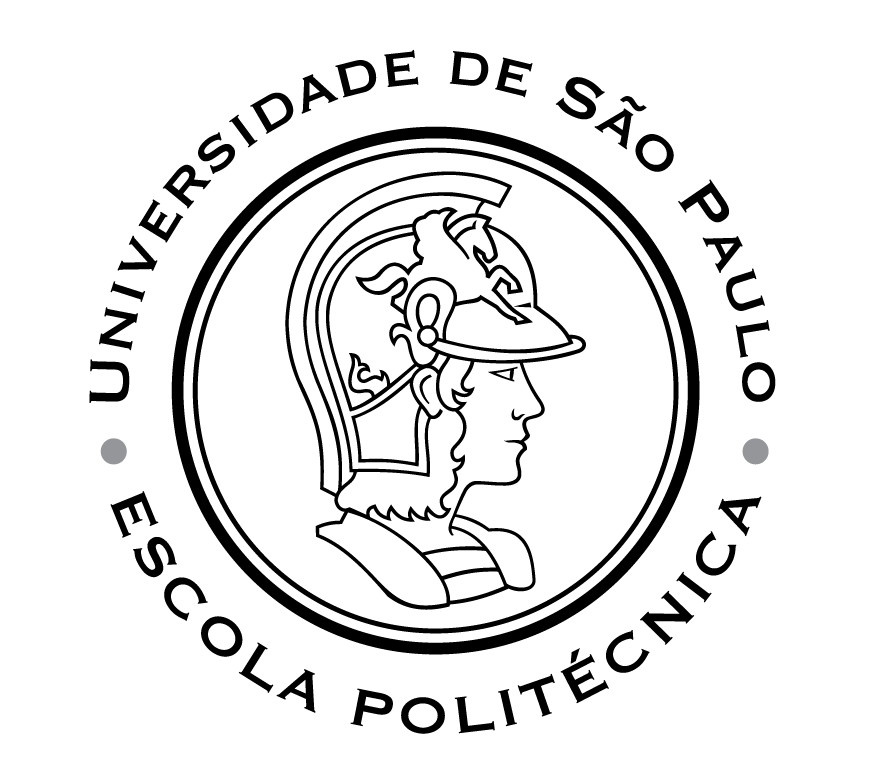
\includegraphics[width=0.8\textwidth]{imagens/Poli.png}
    \caption{Frequência com que os respondentes já desistiram de uma compra por causa da fila, por agrupamento (n = 142).}
    \label{fig:desistencia_cluster}
\end{figure}

\subsubsection{Cluster 1: dependentes de atendimento}

Este foi o maior dos quatro grupos, com 55 de 142 respondentes (39\%). Apresentou a menor pontuação de orientação autonomia-tecnologia-eficiência dos quatro grupos (média de 30,1 em uma escala de 0 a 100) e a maior importância atribuída ao vendedor na hora de experimentar a peça, com concordância unânime nesse item. O comportamento observado combinou baixa sensibilidade a fila (76\% raramente e 22\% nunca desistiram de comprar por causa de fila) com baixa confiança em pagar por celular (73\% discordam ou discordam totalmente) e baixo conhecimento prévio de disponibilidade do produto antes de ir à loja. O contexto típico de compra, segundo as entrevistas associadas a este padrão, envolveu a presença desejada de um vendedor tanto para confirmar a escolha quanto para localizar tamanhos fora da araque. A fricção mais frequente relatada não foi a fila do caixa, e sim a ausência ou demora de um vendedor no momento de escolha e prova. A reação ao conceito de desbloqueio sem checagem manual foi de rejeição quase unânime (96\% discordam ou discordam totalmente, com uma pequena fração neutra e nenhuma concordância).

Este grupo foi, ao mesmo tempo, o mais homogêneo nas duas dimensões usadas para a clusterização e o mais heterogêneo em termos de motivação qualitativa. As entrevistas sugerem que ele reúne ao menos duas motivações distintas por trás de um comportamento de escala semelhante: pessoas que valorizam a companhia e a opinião de um vendedor como parte positiva da experiência, como Marisa, para quem ir à loja funciona como \emph{"um respiro"}, e pessoas que relatam desconfiança de tecnologia e de mudança em si, como Robério, para quem a hipótese de solução \emph{"deixa bem inseguro"} (Entrevista 3). O survey não distingue essas duas motivações; as entrevistas sim. Marisa, sobre o que a faria confiar em um processo sem checagem: \emph{"Confiaria mais se soubesse que tem alguém pra me ajudar caso desse algum problema. Sozinha eu fico insegura"} (Entrevista 1).

\subsubsection{Cluster 2: autônomos digitais}

Este grupo reuniu 30 de 142 respondentes (21\%) e apresentou a maior pontuação de orientação autonomia-tecnologia-eficiência dos quatro grupos (média de 80,8) e a menor importância atribuída ao vendedor na prova (97\% discordam ou discordam totalmente desse item, com 3\% neutro). Foi, simultaneamente, o grupo mais autônomo e o mais incomodado com fila: a totalidade já desistiu de comprar por causa de fila em algum grau, e 17\% relataram isso como algo frequente, a maior taxa entre os quatro grupos. Concentrou a faixa etária mais jovem da amostra (76\% com menos de 35 anos). O contexto típico envolveu uma rotina de tempo apertado, uso corrente de autoatendimento, pagamento por aproximação e pix fora da loja, e busca por velocidade e controle sobre o próprio processo de compra. A fricção mais frequente relatada foi especificamente o tempo perdido em fila, não a dificuldade de achar produto nem a falta de ajuda. A reação ao conceito de desbloqueio sem checagem manual foi a única com aceitação majoritária entre os quatro grupos (100\% concordam ou concordam totalmente, sem nenhuma resposta neutra ou negativa).

Este foi o grupo com maior consistência entre discurso e comportamento relatado: quem afirmou preferir autonomia também foi quem, nas entrevistas correspondentes, efetivamente resolveu a compra sozinho. Thiago, sobre a hipótese de solução: \emph{"Achei sensacional, sinceramente. Resolve exatamente o que eu mais odeio, que é fila"} (Entrevista 6). Felipe, no mesmo sentido, propôs por iniciativa própria estender a ideia para \emph{"avisar estoque em tempo real"} (Entrevista 4), o que indica que, para este grupo, a hipótese de solução foi entendida como potencial ponto de partida para uma integração digital mais ampla, e não apenas como um mecanismo de destravamento.

\subsubsection{Cluster 3: frustrados com disponibilidade}

Este foi o menor dos quatro grupos, com 13 de 142 respondentes (9\%), e o único cujo tamanho coincidiu quase exatamente com o do perfil equivalente na hipótese original de cinco perfis (também 13). Apresentou a maior dor de disponibilidade dos quatro grupos, por larga margem (média de 78,8 em 100, contra 46,5 a 54,5 nos demais grupos), com orientação autonomia-tecnologia-eficiência em nível intermediário-alto (60,6), nem o mais dependente nem o mais autônomo. A totalidade dos respondentes deste grupo relatou sair da loja frequentemente sem comprar por não encontrar o que procurava, e a totalidade discordou de encontrar o tamanho ou a cor que precisava. Foi também o grupo com maior concordância de que saber, pelo aplicativo, se um produto está disponível na loja mudaria sua decisão de se deslocar até ela. A fricção mais frequente relatada foi, de forma consistente, não encontrar tamanho, cor ou modelo, e não fila ou falta de vendedor. A reação ao conceito de desbloqueio sem checagem manual foi de neutralidade praticamente unânime, um padrão distinto dos outros três grupos, nenhum dos quais concentrou-se de forma tão uniforme em um único ponto da escala.

Essa neutralidade unânime é, em si, um dado que exige cautela interpretativa: pode refletir indiferença genuína a um conceito que não tem relação clara com a dor relatada por este grupo, ou pode refletir uma avaliação de fato indiferente. As entrevistas favorecem a primeira leitura. Wagner, comprando para os filhos sem eles presentes, associou-se a este padrão de resposta: \emph{"Achei ok, mas sinceramente não é isso que resolveria meu maior problema, que é acertar o tamanho"}, e, quando perguntado o que a hipótese de solução resolve: \emph{"Resolve uma coisa que nem era meu problema principal. Meu problema é tamanho, isso aqui resolve fila e pagamento"} (Entrevista 10).

\subsubsection{Cluster 4: pragmáticos equilibrados}

Este grupo reuniu 44 de 142 respondentes (31\%), o segundo maior dos quatro, e ocupou posição intermediária em ambas as dimensões usadas para a clusterização: nem alta nem baixa orientação autonomia-tecnologia-eficiência (53,8) e nem alta nem baixa dor de disponibilidade (49,7). O comportamento observado combinou baixa sensibilidade a fila (82\% raramente, 16\% às vezes e 2\% frequentemente desistiram por fila) com posição majoritariamente neutra em praticamente todos os itens de atitude do survey, sem discordância ou concordância forte em nenhum. A reação ao conceito de desbloqueio sem checagem manual foi majoritariamente neutra (91\%), com uma pequena inclinação à concordância (9\%, entre concordo e concordo totalmente) e nenhuma discordância registrada, uma leve tendência à aceitação, não à rejeição.

Por ser o grupo residual das duas dimensões usadas para clusterizar, este é provavelmente o mais heterogêneo internamente em termos de motivação real, e a etiqueta pragmático equilibrado descreve a posição estatística do grupo, não necessariamente uma identidade comportamental compartilhada por todos os 44 respondentes. Vale tratá-lo, nesta etapa, como o que resta depois de isolar os três padrões mais nítidos, não como um perfil positivo e coeso por si. Camila, sobre a hipótese de solução, ilustrou bem essa posição intermediária: \emph{"Achei legal a ideia, principalmente pra quando eu já sei o que quero e não preciso ficar na fila. Mas confesso que não é meu maior problema hoje"} (Entrevista 8), nem rejeição nem entusiasmo.

\subsubsection{Uma pergunta em aberto sobre o quinto perfil original}
\label{sec:cluster_aberto}

A base original foi desenhada com cinco perfis, mas a clusterização convergiu para quatro grupos nítidos. O perfil ausente, cético tradicional, parece ter se fundido ao grupo de menor autonomia (Cluster 1). Duas hipóteses concorrentes explicam essa fusão, e os dados atuais não permitem decidir entre elas. A primeira é que dependência de atendimento e ceticismo tecnológico sejam, de fato, a mesma coisa nesta população: quem depende de vendedor também desconfia de tecnologia, sem que isso represente duas motivações distintas. A segunda é que sejam motivações diferentes, uma de preferência social positiva por interação humana e outra de aversão a risco e mudança, que o instrumento de survey não tem itens específicos para separar, mas que as entrevistas sugerem existirem lado a lado dentro do mesmo cluster, como a diferença entre Marisa, para quem a loja é companhia e cuidado pessoal, e Robério, para quem qualquer novidade tecnológica gera insegurança. Essa questão é retomada na síntese final (Seção~\ref{sec:sintese}).

\subsection{Análise dos resultados da pesquisa quantitativa}
\label{sec:quantitativa}

\subsubsection{O item decisivo: confiança em processo sem checagem manual}

A distribuição de respostas ao item central para a hipótese de solução concentrou-se em discordância e neutralidade: 39\% neutros, 31\% discordam e 6\% discordam totalmente, uma maioria de 76\% que não endossou a ideia. Apenas 24\% concordaram ou concordaram totalmente (Figura~\ref{fig:confianca_geral}). A distribuição não foi bimodal, isto é, não formou dois grupos opostos e nítidos: foi assimétrica, puxada para o lado cético, com uma cauda de concordância bem menor.

\begin{figure}[htbp]
    \centering
    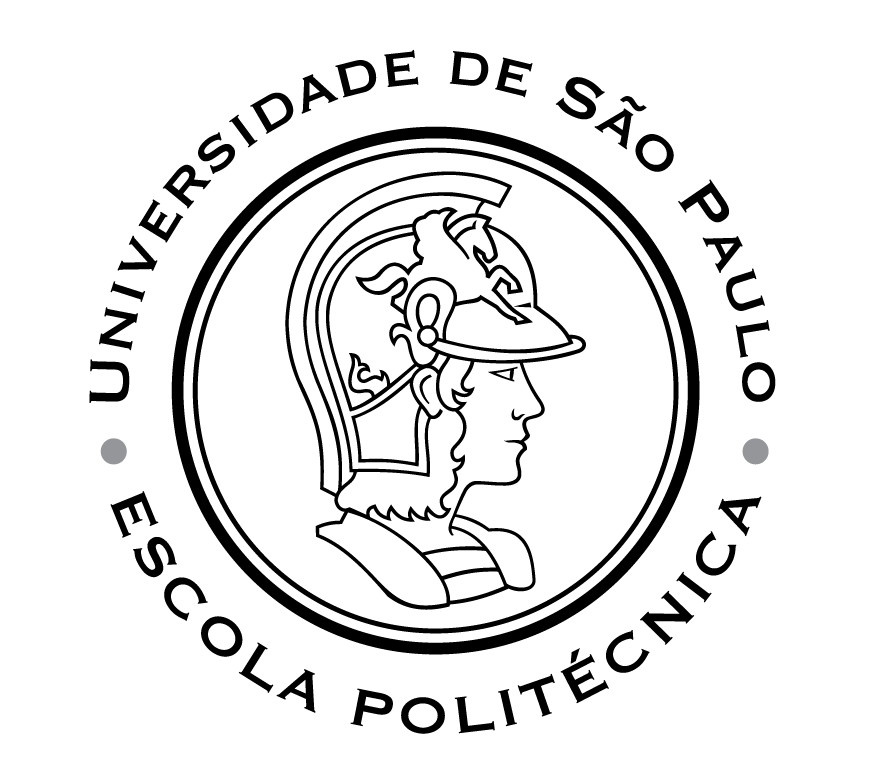
\includegraphics[width=0.8\textwidth]{imagens/Poli.png}
    \caption{Distribuição de respostas ao item de confiança em processo de compra sem checagem manual na saída, desde que o pagamento já esteja confirmado (n = 142).}
    \label{fig:confianca_geral}
\end{figure}

Isso sugere que, nesta amostra, o conceito de dispensar checagem manual não partiu de uma aceitação ampla: encontrou um núcleo relativamente pequeno de interesse claro, os 24\% que concordaram, e uma massa grande que nem rejeitou nem abraçou a ideia. Como mostrado na seção anterior, essa neutralidade não se distribuiu igualmente entre os quatro agrupamentos identificados, e concentrou-se em grupos específicos por motivos qualitativamente diferentes entre si, um caso em que a média geral da amostra esconde mais do que revela.

Neutralidade em um item de escala admite mais de uma leitura: pode indicar indiferença genuína, mas também pode indicar que a pergunta não fez sentido para quem respondeu, por exemplo alguém cuja dor não tem relação com checagem de saída, ou insegurança em avaliar um conceito abstrato sem uma experiência concreta para ancorar a resposta. As entrevistas ajudaram a distinguir essas leituras, e sugerem que, para vários entrevistados, a neutralidade do survey provavelmente escondeu \emph{"isso não resolve o meu problema"}, e não \emph{"não tenho opinião"}.

\subsubsection{Sensibilidade à fila: diferença por agrupamento, não por frequência de compra}

A frequência de compra declarada (algumas vezes ao ano, mensalmente, mais de uma vez por mês) não se associou de forma clara com dor de disponibilidade nem com a orientação autonomia-tecnologia-eficiência: as médias entre grupos de frequência de compra variaram menos de 8 pontos em 100, sem gradiente consistente. Comprar mais, nesta amostra, não tornou a pessoa mais nem menos autônoma, nem mais nem menos incomodada com falta de produto. Quem realmente diferiu foi o agrupamento comportamental: a fração de respondentes que já desistiu de uma compra frequentemente por causa de fila variou de 0\% a 17\% conforme o grupo, e a fração que nunca desistiu variou de 0\% a 22\%.

Essa constatação sugere que a relação entre o cliente e a fila não foi função de quanto ele compra, mas de um padrão comportamental mais amplo, o mesmo eixo de orientação autonomia-tecnologia-eficiência discutido na Seção~\ref{sec:clusters}. Essa leitura contraria a suposição de que a fila representa uma fricção universal e uniforme entre os clientes: os dados sugerem algo mais específico, fila incomodou intensamente, mas principalmente um segmento identificável da amostra, não a amostra como um todo. Vale registrar que frequência de compra é uma medida autodeclarada que não distingue ida à loja de compra efetiva: alguém que visita a loja com frequência para navegar, como o comportamento relatado por Luana, pode responder mensalmente mesmo comprando raramente.

\subsubsection{Disponibilidade de tamanho e cor: um problema concentrado, não disperso}

Olhando a amostra inteira, a maioria das respostas ao item sobre encontrar o tamanho ou a cor desejada se concentrou em torno de neutro, o que poderia sugerir um problema brando e disperso. Ao segmentar por agrupamento comportamental, no entanto, emergiu um grupo pequeno (13 de 142, 9\% da amostra) no qual a totalidade dos respondentes discordou ou discordou totalmente desse item, e a totalidade relatou sair da loja frequentemente sem comprar por não encontrar o que procurava, o oposto do padrão do restante da amostra. A leitura de que disponibilidade não é um problema generalizado mudou quando o dado foi desagregado: o problema existiu, mas concentrado com intensidade alta em um subgrupo específico, e quase ausente no resto da amostra, um padrão que a média geral escondeu e que a segmentação revelou. Com apenas 13 respondentes, esse subgrupo é pequeno demais para generalizações de proporção populacional, mesmo dentro dos limites já postos pelo tamanho e pela representatividade incerta da amostra. Seu valor aqui é qualitativo: mostrar que o padrão existiu e foi internamente consistente, não estimar que fração real de clientes da Riachuelo ele representa.

\subsubsection{Orientação autonomia-tecnologia-eficiência por faixa etária}

Houve uma tendência de queda na orientação autonomia-tecnologia-eficiência conforme a idade aumentou, de uma média de 62 (em escala de 0 a 100) entre 18 e 24 anos até valores entre 40 e 45 a partir dos 45 anos, mas a diferença entre faixas adjacentes foi pequena diante da dispersão dentro de cada faixa (Figura~\ref{fig:idade}). Existe, portanto, uma associação, mas fraca e gradual, e não um corte nítido entre jovem autônomo e idoso dependente. A dispersão dentro de cada faixa etária foi grande o bastante para que um respondente de 60 anos pontuasse mais alto em autonomia e tecnologia do que um de 25, e as entrevistas confirmaram isso com casos concretos: Nivaldo, aposentado, relatou testar autoatendimento sem problema, enquanto Débora, mais jovem, relatou depender fortemente de uma vendedora específica. Usar idade como preditor único de orientação a autonomia, a partir deste gráfico isoladamente, forçaria uma generalização que os próprios dados não sustentam: a idade parece contribuir para essa orientação, mas não a determina.

\begin{figure}[htbp]
    \centering
    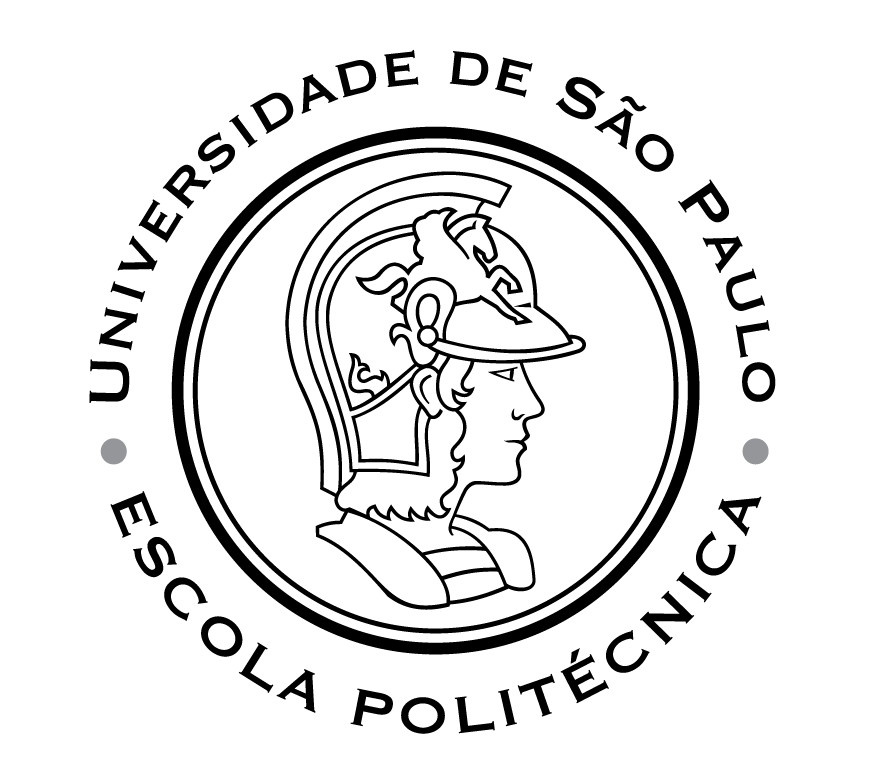
\includegraphics[width=0.8\textwidth]{imagens/Poli.png}
    \caption{Orientação autonomia-tecnologia-eficiência por faixa etária (n = 142).}
    \label{fig:idade}
\end{figure}

\subsubsection{Qualidade e limitações da base quantitativa}

Alguns itens do survey apresentaram pouca variação e, por isso, pouca utilidade para diferenciar respondentes: consigo encontrar facilmente os produtos que procuro (82\% neutro), encontro o tamanho ou a cor que preciso (87\% neutro), um vendedor te aborda com que frequência (92\% às vezes), já me senti desconfortável com verificação na saída (99\% nunca ou raramente). Esses itens foram mantidos na base, mas pesaram pouco nas dimensões construídas. Os itens com melhor variação, e por isso mais informativos, foram os cinco itens do bloco de autonomia e atendimento, os três itens de confiança em tecnologia, e o item decisivo de aceitação do desbloqueio sem checagem manual, sobre os quais a análise de clusters se apoiou.
\subsection{Análise das entrevistas qualitativas}
\label{sec:qualitativa}

Esta seção aprofunda padrões que o survey, por sua natureza fechada, não capturou sozinho. A leitura das onze entrevistas foi conduzida tema a tema, e não entrevista a entrevista, para permitir comparação direta entre relatos.

\subsubsection{Contradição entre autonomia na prova e dependência na busca}

Como já indicado na Seção~\ref{sec:caracterizacao}, vários entrevistados relataram, na mesma conversa, preferir resolver sozinhos uma etapa da jornada e depender fortemente de ajuda em outra, sem tratar isso como contradição. Esse achado qualitativo é relevante porque sugere que autonomia não é uma preferência de traço único, como o survey a trata ao reduzi-la a um único conjunto de itens agregados, e sim uma preferência que varia conforme a etapa da jornada, especificamente cedendo lugar à dependência de ajuda quando o produto procurado não está visível ou disponível.

\subsubsection{Perder contato com quem ajuda pesa mais que falha técnica, para quem já depende de ajuda}

Uma das perguntas finais do roteiro pediu que o entrevistado escolhesse entre dois receios: a tecnologia falhar, ou perder contato com alguém que ajuda quando precisa. A resposta divergiu de forma consistente com o padrão comportamental do entrevistado, e não pareceu uma preocupação universal. Marisa respondeu: \emph{"Perder o contato com quem ajuda, com certeza. Pra mim isso é mais importante que a tecnologia funcionar direitinho"} (Entrevista 1). Wagner respondeu de forma equivalente: \emph{"Perder contato com quem ajuda, porque é dessa ajuda que eu mais preciso, mais do que da tecnologia em si"} (Entrevista 10). Thiago, no extremo oposto de autonomia, sequer tratou isso como dilema, e não mencionou a possibilidade de precisar de ajuda ao reagir à hipótese de solução. Isso indica que a resistência à ideia de destravamento remoto, onde apareceu, não foi necessariamente resistência à tecnologia em si (falha técnica), e sim resistência a perder um vínculo de suporte que a pessoa já usa e valoriza hoje.

\subsubsection{Risco reputacional: o medo de ser mal interpretado}

Uma nuance apareceu de forma explícita em apenas uma entrevista, mas merece registro por descrever um tipo de preocupação distinto de falha técnica. Marisa relatou: \emph{"Fico pensando, e se der algum erro e a etiqueta não destravar, ou pior, destravar errado e eu ser acusada de estar levando sem pagar? Isso me preocupa mais do que me anima, sinceramente"} (Entrevista 1). Essa fala descreveu um risco reputacional e social, o de ser vista como estivesse furtando, distinto do risco técnico de o sistema não funcionar e do risco financeiro de ser cobrada de forma incorreta, mencionado por Robério em relação a autoatendimento de supermercado (Entrevista 3). Os três tipos de risco parecem coexistir nas entrevistas, sem que os dados atuais indiquem qual pesa mais para o conjunto da amostra: o survey não tem item específico para risco reputacional, uma lacuna a registrar como hipótese em aberto, não uma conclusão a forçar.

\subsubsection{O vendedor como pessoa nomeada, não como função genérica}

Em duas entrevistas, a relação com o vendedor não foi descrita como atendimento genérico, e sim como relação pessoal com alguém específico, ao ponto de a entrevistada nomeá-la. Débora, sobre a vendedora que a atende há dois anos: \emph{"Ela filtra as opção pra mim, eu tenho pouco tempo, então isso é essencial, evita eu perder tempo vendo coisa que não combina"}, e, sobre a hipótese de solução: \emph{"Fico com um pé atrás, viu, porque isso parece tirar justamente a parte que eu mais valorizo, que é a pessoa envolvida no processo"} (Entrevista 9). Renata descreveu uma relação equivalente com sua consultora fixa, e distinguiu explicitamente entre usar uma solução mais autônoma \emph{"pra uma reposição rápida"} (aceitável) e usar em uma compra que envolve escolha completa com a consultora (não substituível, Entrevista 7). Esse padrão, vendedor como relação individual não intercambiável, é qualitativamente diferente da dependência de atendimento genérica medida pelo survey, e ajuda a explicar por que o Cluster 1 (dependentes de atendimento) reuniu tanto motivação de conforto e insegurança, como em Marisa e Robério, quanto motivação de relação de confiança construída ao longo do tempo, como em Débora e Renata.

\subsubsection{Uma entrevistada fora da curva}

Luana, estudante de moda que entra em lojas quase toda semana mas compra a cada dois ou três meses, não se encaixou com conforto em nenhum dos quatro agrupamentos descritos na Seção~\ref{sec:clusters}. Apresentou alta autonomia, quase nunca buscando vendedor, mas não por eficiência ou pressa, e sim por preferência de observar sozinha, sem meta de compra definida. Sua reação à hipótese de solução foi reveladora dessa diferença: \emph{"Não resolve nada do que eu mencionei, resolve um problema que eu acho que é mais de outro tipo de cliente, não o meu caso"} (Entrevista 11). Luana foi também a única entrevistada a levantar uma preocupação de dados e privacidade em relação à etiqueta inteligente, \emph{"penso em quanto dado estão coletando sobre isso"}, tema que nenhum outro entrevistado mencionou e que o survey não investigou diretamente. Esse é um sinal isolado, não um padrão, mas um sinal que a análise não deveria descartar apenas por aparecer uma única vez.

\subsection{Integração entre evidências quantitativas e qualitativas}
\label{sec:integracao}

Os quatro agrupamentos identificados na Seção~\ref{sec:clusters} encontraram correspondência razoável nas entrevistas, mas a correspondência não foi perfeita, e as diferenças foram informativas.

O Cluster 1 (dependentes de atendimento) correspondeu a Marisa, Robério, Débora e, parcialmente, Renata. O survey mostrou rejeição quase unânime ao conceito de desbloqueio sem checagem neste grupo; as entrevistas explicaram o porquê, com nuance que o survey não capturou: Robério rejeitou por desconfiança de tecnologia e mudança, Marisa rejeitou por medo de ficar sem suporte caso algo desse errado, e Débora rejeitou porque a proposta reduziria o papel da pessoa que ela mais valoriza no processo. Três motivos distintos produziram a mesma resposta de escala, exatamente o tipo de heterogeneidade já sinalizado na Seção~\ref{sec:cluster_aberto}.

O Cluster 2 (autônomos digitais) correspondeu a Thiago e Felipe de forma mais direta: o survey mostrou aceitação total e a maior taxa de desistência por fila entre os quatro grupos; as entrevistas mostraram os mesmos dois entrevistados relatando episódios concretos de desistência por fila (Black Friday, hora de almoço) e reação entusiasmada ao conceito, sem ressalva relevante. Foi o cluster onde discurso, comportamento relatado e reação ao conceito mais convergiram.

O Cluster 3 (frustrados com disponibilidade) correspondeu a Wagner e, parcialmente, a Nivaldo. O survey isolou um grupo pequeno e nitidamente definido por dificuldade de achar tamanho ou cor; Wagner confirmou esse padrão de forma direta, com uma causa específica, comprar para os filhos sem eles presentes, que o survey não captura como variável mas que produziu o mesmo padrão de resposta. Nivaldo se aproximou parcialmente deste grupo, já que sua queixa central também foi disponibilidade (tamanhos maiores), embora tivesse sido originalmente associado ao perfil de eficiência, não ao de disponibilidade. Esse é um exemplo direto de um perfil original sendo contrariado pelo comportamento relatado.

O Cluster 4 (pragmáticos equilibrados) correspondeu a Camila e, parcialmente, a Joyce. O grupo residual do survey, com posição intermediária em tudo, encontrou em Camila uma ilustração razoável: reação morna ao conceito, sem fricção aguda relatada, fila tolerada fora de datas especiais. Joyce se encaixou apenas parcialmente, sendo mais eficiente e apressada do que a média deste cluster sugeriria, o que é coerente com o próprio survey mostrar este grupo como o mais heterogêneo internamente.

Duas coisas apareceram nas entrevistas sem equivalente claro na estrutura de quatro grupos do survey, e vale destacá-las em vez de forçar seu encaixe: a relação nomeada com um vendedor específico (Débora, Renata), qualitativamente distinta de concordar com o item sobre importância do vendedor, e o perfil de baixa frequência e alta autonomia por desinteresse, não por eficiência (Luana), que não se explicou bem por nenhuma combinação das duas dimensões usadas na clusterização. Ambas ficam registradas como limite do que a segmentação quantitativa, isoladamente, conseguiu capturar.
\subsection{Necessidades, desejos e demandas dos clientes}
\label{sec:ndd}

\subsubsection{Nota metodológica}

Esta seção traduziu os achados das Seções~\ref{sec:caracterizacao} a \ref{sec:integracao} em formulações de necessidade, desejo e demanda, seguindo a distinção clássica de Kotler entre necessidade (estado em que se percebe alguma privação), desejo (necessidade humana moldada pela cultura e por características individuais, que pode ser representada por diferentes bens capazes de satisfazê-la) e demanda (desejo associado a um contexto concreto de comportamento, disposição de compra ou expectativa explicitamente manifestada). Operacionalmente, esta análise tratou como necessidade uma condição ou resultado que o cliente valorizou como relevante para realizar a jornada de compra de forma adequada; como desejo uma preferência ou expectativa cuja ausência não impede a compra nem gera uma falha fundamental na experiência; e como demanda uma necessidade ou desejo associado a um comportamento recorrente, um contexto concreto de compra ou uma expectativa explicitamente manifestada pelo entrevistado. A classificação evitou um erro comum: tratar como demanda um item apenas porque a fala que o sustenta foi emocionalmente intensa. Intensidade de fala não equivale a demanda; o critério usado foi a presença de um comportamento concreto e recorrente por trás da fala, não o tom em que ela foi dita.

Cada item a seguir foi formulado na perspectiva do resultado desejado pelo cliente, independentemente da hipótese de solução em estudo, e não foi tratado como requisito de produto. Itens semelhantes, mas associados a contextos, comportamentos ou benefícios distintos, foram mantidos separados, sem consolidação prematura. A matriz da Seção~\ref{sec:matriz} reúne todos os itens com sua rastreabilidade às evidências.

\subsubsection{Necessidades identificadas}

\textbf{N01. Ter apoio humano disponível para confirmar decisões de compra e auxiliar na experimentação da peça.} Associada principalmente ao Cluster 1 (dependentes de atendimento, 39\% da amostra) e, com menor intensidade, ao Cluster 4. Evidência quantitativa: concordância unânime com a importância do vendedor na prova e 96\% de rejeição ao item de confiança em processo sem checagem, ambos no Cluster 1. Evidência qualitativa: Marisa (Entrevista 1) descreveu a loja como um momento em que confia menos no próprio julgamento sem uma opinião externa; Robério (Entrevista 3) relatou que, sem vendedor disponível, provavelmente sairia sem comprar. Contexto: momento de escolha e experimentação da peça. Interpretação: para este grupo, a presença de um vendedor não funciona apenas como recurso instrumental para achar tamanho, mas como parte do valor da experiência ou da confiança na própria decisão. Contradição: dentro do mesmo cluster coexistem motivações distintas, uma de sociabilidade positiva e outra de aversão a risco e mudança (Seção~\ref{sec:cluster_aberto}), o que a formulação única desta necessidade não distingue. Limitação: o survey mede importância do vendedor com um único item, insuficiente para separar essas duas motivações.

\textbf{N02. Ter garantia de que existe apoio disponível caso algo dê errado em um processo de compra menos assistido.} Associada ao Cluster 1. Evidência quantitativa: 96\% de rejeição ao item de confiança em processo sem checagem manual no Cluster 1. Evidência qualitativa: quando confrontados com a escolha entre tecnologia falhar e perder contato com quem ajuda, Marisa, Robério e Wagner priorizaram o segundo receio (Entrevistas 1, 3 e 10); Marisa declarou diretamente que perder esse contato \emph{"é mais importante que a tecnologia funcionar direitinho"}. Contexto: qualquer processo de compra com menor mediação humana. Interpretação: a resistência a processos menos assistidos, onde presente, parece relacionar-se menos ao funcionamento técnico da solução e mais ao risco de ficar sem a quem recorrer. Contradição: Thiago (Entrevista 6), do Cluster 2, não tratou essa escolha como dilema relevante, o que reforça que esta necessidade não é transversal à amostra. Limitação: a pergunta que originou essa evidência foi feita apenas na etapa final da entrevista, depois de o conceito de solução já ter sido apresentado, o que pode ter induzido a resposta.

\textbf{N03. Encontrar o tamanho, a cor ou o modelo procurado dentro de um esforço razoável.} Associada principalmente ao Cluster 3 (frustrados com disponibilidade, 9\% da amostra), presente em menor grau nos demais clusters. Evidência quantitativa: no Cluster 3, totalidade dos respondentes discorda de encontrar o tamanho ou a cor que precisa, e totalidade relata sair da loja frequentemente sem comprar por esse motivo. Evidência qualitativa: Marisa (Entrevista 1) relatou que essa dificuldade é \emph{"bem frequente"} para o próprio tamanho; Nivaldo (Entrevista 5) atribuiu a mesma dificuldade à própria estatura acima da média. Contexto: busca de produto dentro da loja, antes de qualquer decisão de compra. Interpretação: esta necessidade é intensa e concentrada em um subgrupo pequeno e nitidamente definido, e quase ausente no restante da amostra, um padrão que a média geral do survey esconde. Contradição: nenhuma identificada além da concentração já descrita. Limitação: com apenas 13 respondentes no Cluster 3, o valor desta evidência é qualitativo, não uma estimativa de proporção populacional.

\textbf{N04. Obter ajuda para localizar uma peça que não está exposta ou disponível na araca de venda.} Transversal, mais forte nos Clusters 1 e 3. Evidência quantitativa: item de importância do vendedor concentrado em concordância no Cluster 1; correlação entre dor de disponibilidade e busca de ajuda relatada nas entrevistas. Evidência qualitativa: Marisa (Entrevista 1), Camila (Entrevista 8) e Nivaldo (Entrevista 5) relataram recorrer a um vendedor especificamente para verificar estoque quando o item não estava na araca. Contexto: ocorre depois de uma busca inicial sem sucesso pelo próprio cliente. Interpretação: esta necessidade é distinta de N01, já que não envolve apoio à decisão, e sim acesso a um estoque que o cliente sozinho não alcança. Contradição: nenhuma identificada. Limitação: o survey não distingue estoque em araca de estoque em depósito, o que limita a precisão desta leitura.

\textbf{N05. Confiar que a informação de estoque exibida em canais digitais corresponde à realidade da loja física.} Transversal, evidência concentrada nas entrevistas. Evidência quantitativa: não medida diretamente pelo survey, uma lacuna do instrumento. Evidência qualitativa: Joyce (Entrevista 2), Felipe (Entrevista 4) e Renata (Entrevista 7) relataram, de forma independente, ter perdido confiança na informação de estoque de site ou aplicativo após uma divergência entre o que viram online e o que encontraram na loja. Contexto: pesquisa prévia à visita à loja. Interpretação: uma parte da amostra parte de uma credibilidade já corroída em relação a canais digitais de disponibilidade, e não de uma expectativa neutra, o que qualquer solução futura que dependa de exibir disponibilidade pelo aplicativo precisaria reconstruir. Contradição: nenhuma identificada. Limitação: evidência qualitativa isolada, sem contraparte quantitativa; não é possível estimar sua prevalência na base de clientes.

\textbf{N06. Concluir a compra sem risco de ser mal interpretado ou constrangido por uma falha ou checagem no momento da saída.} Transversal, mais saliente no Cluster 1. Evidência quantitativa: o item de desconforto com verificação na saída apresentou pouca variação na amostra (99\% nunca ou raramente), o que limita sua capacidade de diferenciar respondentes, mas não descarta a preocupação em si. Evidência qualitativa: Marisa (Entrevista 1) relatou temer ser \emph{"acusada de estar levando sem pagar"} em caso de falha; Joyce (Entrevista 2) descreveu incômodo com a checagem de nota na saída, \emph{"parece que estão desconfiando de mim"}. Contexto: momento de saída da loja. Interpretação: este é um risco reputacional e social, distinto de falha técnica ou erro de cobrança, que o survey não mediu com item específico. Contradição: nenhuma identificada. Limitação: evidência qualitativa concentrada em duas entrevistas; permanece como hipótese sobre sua prevalência real na base de clientes.

\textbf{N07. Comprar corretamente para terceiros sem poder verificar o ajuste no corpo da pessoa.} Contexto específico, associado parcialmente ao Cluster 3. Evidência quantitativa: o survey não identifica para quem a peça está sendo comprada, uma lacuna do instrumento. Evidência qualitativa: toda a Entrevista 10 (Wagner) descreveu essa insegurança de forma consistente, incluindo a estratégia de fotografar etiquetas em casa antes de sair e levar duas opções de tamanho para garantir. Contexto: compra de roupas infantis ou para outro adulto, sem a pessoa presente. Interpretação: esta necessidade tem natureza diferente da dificuldade geral de encontrar tamanho (N03), já que a incerteza recai sobre uma variável que o comprador não controla, o corpo de terceiros, e não sobre a disponibilidade do produto. Contradição: nenhuma identificada. Limitação: evidência de uma única entrevista; não é possível estimar, com os dados atuais, que fração da amostra vive situação semelhante.

\textbf{N08. Preservar a opção de contar com atendimento humano mesmo quando existem alternativas de autoatendimento.} Associada ao Cluster 1 e a parte do Cluster 4, presente inclusive entre entrevistados com alta confiança em tecnologia. Evidência quantitativa: rejeição concentrada ao item de confiança sem checagem no Cluster 1, ainda que outros itens de confiança em tecnologia deste grupo não sejam uniformemente baixos. Evidência qualitativa: Renata (Entrevista 7), que relatou confiar tecnicamente em pagamento por celular, afirmou preferir que uma solução mais autônoma fosse \emph{"opcional, que não substituísse a possibilidade de ter uma pessoa por perto"}; Débora (Entrevista 9) pediu que a vendedora permanecesse envolvida \emph{"nem que fosse ela confirmando pelo sistema dela que está tudo certo"}. Interpretação: esta necessidade distingue-se de N01 e N02 por não depender de baixa confiança em tecnologia, e sim de uma preferência por manter a opção de atendimento, mesmo entre quem já demonstra autonomia tecnológica em outros contextos. Contradição: aparente, já que Renata e Débora pontuam relativamente alto em confiança tecnológica mas ainda assim priorizam esta necessidade, o que indica que autonomia tecnológica e preferência por manter atendimento humano não são mutuamente excludentes nesta amostra. Limitação: evidência concentrada em duas entrevistas específicas, ambas de clientes com relação nomeada com uma vendedora (Seção~\ref{sec:qualitativa}).

\subsubsection{Desejos identificados}

\textbf{D01. Escolher e experimentar produtos sem abordagem insistente de vendedores.} Associada aos Clusters 2 e 4, presente também no Cluster 1 em situações específicas. Evidência quantitativa: baixa importância atribuída ao vendedor na prova no Cluster 2 (97\% discordam ou discordam totalmente). Evidência qualitativa: Thiago (Entrevista 6), Felipe (Entrevista 4), Camila (Entrevista 8), Luana (Entrevista 11) e Nivaldo (Entrevista 5) relataram desconforto com vendedores insistentes durante a exploração da loja. Contexto: momento de busca e exploração, antes da decisão de compra. Interpretação: a ausência desse desejo não impediu nenhuma compra relatada, mas sua presença piorou a experiência quando violada, o que o qualifica como desejo, e não necessidade. Contradição: Nivaldo, do Cluster 1, também relatou esse desejo, ainda que valorize apoio em outras etapas, o que reforça a leitura de autonomia variável por etapa da jornada (Seção~\ref{sec:caracterizacao}). Limitação: o survey não mede diretamente frequência ou insistência de abordagem, apenas a frequência declarada de abordagem em geral.

\textbf{D02. Obter uma segunda opinião confiável sobre caimento em compras de maior formalidade ou valor.} Contextual, associada a Felipe (Cluster 2) e Renata (Cluster 4, fronteira). Evidência qualitativa: Felipe (Entrevista 4) relatou pedir opinião para roupas sociais, mas resolver sozinho itens básicos; Renata (Entrevista 7) relatou intensificar o uso da consultora para peças de valor mais alto. Contexto: compra de peças formais ou de maior valor. Interpretação: este desejo é condicional ao tipo de peça, não constante, o que o distingue de N01, associada a um padrão comportamental estável. Contradição: nenhuma identificada, mas o padrão é relevante porque mostra que mesmo clientes de alta autonomia podem desejar apoio pontual. Limitação: evidência de apenas duas entrevistas; o survey não segmenta a importância do vendedor por tipo de peça.

\textbf{D03. Ter confirmação clara e imediata de que o pagamento foi processado corretamente.} Transversal. Evidência qualitativa: Joyce (Entrevista 2) pediu \emph{"algum aviso, tipo pode sair, tá tudo certo"}; Nivaldo (Entrevista 5) mencionou desejar \emph{"um comprovante bem claro"}. Contexto: qualquer processo de pagamento, assistido ou não. Interpretação: este desejo aparece como condição de conforto, não como barreira que impeça a compra, distinguindo-se de N02, que envolve garantia de suporte em caso de falha, não apenas confirmação de sucesso. Contradição: nenhuma identificada. Limitação: evidência qualitativa; o survey não testa formatos de confirmação.

\textbf{D04. Contar com uma relação de confiança contínua com um vendedor específico que conhece o próprio estilo.} Específica, associada a Débora e Renata. Evidência qualitativa: Débora (Entrevista 9) descreveu dois anos de relação com a mesma vendedora, e relatou frustração quando atendida por outra pessoa; Renata (Entrevista 7) descreveu sua vendedora como \emph{"praticamente uma consultora de estilo"}. Contexto: compras recorrentes na mesma unidade. Interpretação: este desejo é qualitativamente distinto de N01, já que não se satisfaz com qualquer atendimento humano disponível, apenas com a continuidade de uma relação específica. Contradição: nenhuma identificada. Limitação: evidência de apenas duas entrevistas; o survey não captura relação nomeada com vendedor, apenas importância genérica de atendimento.

\textbf{D05. Ter uma ferramenta ou orientação que ajude a estimar corretamente o tamanho de terceiros.} Contextual, associada a Wagner. Evidência qualitativa: Wagner (Entrevista 10) sugeriu diretamente \emph{"alguma tabela melhor ou algo que me ajudasse a acertar de primeira"}. Contexto: compra para filhos sem eles presentes. Interpretação: este desejo é complementar a N07, mas distinto dela: enquanto N07 descreve a condição de incerteza, D05 descreve uma solução específica que o próprio cliente propôs, sem que sua ausência tenha impedido a compra relatada (ele resolveu levando duas opções). Contradição: nenhuma identificada. Limitação: evidência de uma única entrevista.

\textbf{D06. Vivenciar a visita à loja como um momento de lazer e exploração sem pressão de tempo.} Associada aos Clusters 4 e a parte do Cluster 1 (Marisa), presente com força em Camila e Luana. Evidência qualitativa: Camila (Entrevista 8) descreveu a compra como \emph{"mais um programa do que uma obrigação"}; Luana (Entrevista 11) tratou a entrada em lojas como observação profissional, não como tarefa de compra. Contexto: visitas sem objetivo de compra definido. Interpretação: este é um desejo contextual, presente apenas quando a visita não é orientada a uma necessidade pontual, o que o distingue de necessidades ligadas a jornadas de reposição rápida. Contradição: nenhuma identificada. Limitação: o survey não distingue visitas exploratórias de visitas orientadas a resultado.

\textbf{D07. Ter privacidade quanto aos próprios dados de comportamento em interações com produtos conectados.} Sinal isolado, associado a Luana. Evidência qualitativa: Luana (Entrevista 11) relatou desconforto ao imaginar uma peça que \emph{"soubesse"} onde está ou quem a manuseou, \emph{"penso em quanto dado estão coletando sobre isso"}. Contexto: qualquer tecnologia que rastreie interação do cliente com o produto. Interpretação: mantido como desejo isolado, não como padrão, dada a ausência de qualquer menção equivalente nas outras dez entrevistas ou no survey. Contradição: nenhuma. Limitação: evidência de menção única; não deve ser descartada apenas por isso, mas também não deve ser generalizada.

\subsubsection{Demandas identificadas}

\textbf{DE01. Reduzir o tempo de espera no caixa em períodos de alta demanda.} Associada ao Cluster 2 (autônomos digitais). Evidência quantitativa: 17\% do Cluster 2 relatou desistir de compra por fila \emph{"frequentemente"}, a maior taxa entre os quatro grupos, e a totalidade do grupo já desistiu em algum grau. Evidência qualitativa: Thiago (Entrevista 6) relatou episódio concreto em uma Black Friday; Felipe (Entrevista 4) relatou episódio concreto durante o horário de almoço, com cálculo explícito de tempo disponível antes de desistir. Contexto: dias de promoção, fins de semana e horários de pico, especialmente almoço. Interpretação: esta é uma demanda no sentido operacional adotado aqui, um desejo associado a um comportamento recorrente e mensurável de abandono de compra, e não apenas uma preferência declarada. Contradição: nenhuma. Limitação: a magnitude da demanda depende de loja e horário específicos, não quantificados no survey.

\textbf{DE02. Ampliar o número de cabines de provador disponíveis em dias de alta demanda.} Associada a Marisa (Cluster 1). Evidência qualitativa: Marisa (Entrevista 1) relatou fila de provador como recorrente, \emph{"bem parecido, quase sempre que eu vou tem fila de provador, principalmente fim de semana"}, e recomendou diretamente mais cabines em dias de promoção. Contexto: dias de promoção e fins de semana. Interpretação: esta demanda foi mencionada de forma explícita e ligada a um comportamento recorrente relatado (espera de provador em quase toda visita), o que a diferencia de um desejo genérico de conforto. Contradição: nenhuma. Limitação: evidência de uma única entrevista; o survey não mede fila de provador separadamente de fila de caixa.

\textbf{DE03. Aumentar a disponibilidade de vendedores em dias de promoção e fins de semana.} Associada aos Clusters 1. Evidência qualitativa: Marisa e Robério (Entrevistas 1 e 3) pediram explicitamente mais vendedores nos períodos de maior movimento, ligando o pedido a episódios concretos de espera sem atendimento disponível. Contexto: dias de promoção, especialmente perto do provador. Interpretação: demanda ligada a um contexto operacional recorrente, coerente com N01, mas formulada como ajuste de capacidade, não como preferência geral por atendimento. Contradição: nenhuma. Limitação: evidência qualitativa; o survey não mede disponibilidade de vendedores por dia ou horário.

\textbf{DE04. Saber, antes de se deslocar até a loja, se o produto desejado está disponível naquela unidade.} Associada principalmente ao Cluster 3. Evidência quantitativa: totalidade do Cluster 3 concordou que saber pelo aplicativo se um produto está disponível mudaria sua decisão de se deslocar até a loja, a maior concentração de concordância nesse item entre os quatro grupos. Evidência qualitativa: Wagner (Entrevista 10), Joyce (Entrevista 2), Felipe (Entrevista 4) e Marisa (Entrevista 1) mencionaram espontaneamente que essa informação mudaria seu comportamento. Contexto: planejamento da visita à loja. Interpretação: esta demanda combina evidência quantitativa forte em um subgrupo específico com evidência qualitativa transversal, o que a torna uma das mais robustas desta análise, ainda que sua intensidade varie por cluster. Contradição: nenhuma. Limitação: depende de resolver antes a necessidade de confiança em canais digitais (N05), sem a qual essa informação pode não ser usada mesmo quando disponível.

\textbf{DE05. Ter uma opção de pagamento rápida para compras simples, sem abrir mão de atendimento em compras mais elaboradas.} Associada aos Clusters 1 e 4. Evidência qualitativa: Renata (Entrevista 7) distinguiu explicitamente entre usar uma solução mais autônoma \emph{"pra uma reposição rápida"} e recusar essa mesma solução em uma compra que envolve consultoria completa; Camila (Entrevista 8) fez distinção semelhante entre reposição de básico e o clima de passear pela loja. Contexto: presença simultânea de dois tipos de compra no repertório do mesmo cliente. Interpretação: esta demanda é condicional ao tipo de compra dentro da jornada do mesmo cliente, e não uma preferência fixa por rapidez ou por atendimento, o que a distingue de DE01 (fila como fricção geral do Cluster 2) e de N01 (apoio humano como necessidade estável do Cluster 1). Contradição: aparente à primeira vista, já que os mesmos clientes que valorizam atendimento (N01, N08) também relataram, em contexto específico, preferência por rapidez, o que reforça que a preferência por autonomia ou assistência depende do contexto da compra, e não apenas do perfil do cliente. Limitação: evidência de duas entrevistas; o survey não segmenta por tipo de compra dentro da jornada do mesmo respondente.
\subsubsection{Matriz consolidada de necessidades, desejos e demandas}
\label{sec:matriz}

A Tabela~\ref{tab:matriz_ndd} consolida os itens apresentados, preservando a rastreabilidade entre cada formulação e a evidência que a originou. A tabela requer o pacote \texttt{pdflscape} (ambiente \texttt{landscape}) e os pacotes \texttt{longtable} e \texttt{array} no preâmbulo do documento principal, dada a largura de conteúdo.

\footnotesize
\begin{longtable}{p{0.9cm} p{1.9cm} p{4.2cm} p{2.4cm} p{3.5cm} p{3.5cm} p{2.4cm} p{3.3cm}}
\caption{Matriz consolidada de necessidades, desejos e demandas dos clientes, com rastreabilidade às evidências.} \label{tab:matriz_ndd} \\
\toprule
\textbf{ID} & \textbf{Tipo} & \textbf{Formulação} & \textbf{Cluster associado} & \textbf{Evidência quantitativa} & \textbf{Evidência qualitativa} & \textbf{Contexto} & \textbf{Observações} \\
\midrule
\endfirsthead
\multicolumn{8}{c}{\textbf{Tabela~\ref{tab:matriz_ndd} (continuação)}} \\
\toprule
\textbf{ID} & \textbf{Tipo} & \textbf{Formulação} & \textbf{Cluster associado} & \textbf{Evidência quantitativa} & \textbf{Evidência qualitativa} & \textbf{Contexto} & \textbf{Observações} \\
\midrule
\endhead
\midrule
\multicolumn{8}{r}{\textit{continua na próxima página}} \\
\endfoot
\bottomrule
\endlastfoot
N01 & Necessidade & Ter apoio humano disponível para confirmar decisões e auxiliar na experimentação & Cluster 1; parcial Cluster 4 & 100\% concordam importância do vendedor na prova; 96\% rejeitam compra sem checagem (Cluster 1) & Marisa (Entr. 1); Robério (Entr. 3); Débora (Entr. 9) & Escolha e prova da peça & Cluster heterogêneo; duas motivações distintas coexistem (Seção~\ref{sec:cluster_aberto}) \\
N02 & Necessidade & Ter garantia de apoio disponível caso algo dê errado em processo menos assistido & Cluster 1 & 96\% rejeitam compra sem checagem (Cluster 1) & Marisa, Robério, Wagner priorizam ``perder contato'' sobre falha técnica (Entr. 1, 3, 10) & Processos com menor mediação humana & Pergunta feita após apresentação do conceito, risco de indução \\
N03 & Necessidade & Encontrar o tamanho, a cor ou o modelo procurado dentro de esforço razoável & Cluster 3 & 100\% discordam de encontrar tamanho/cor; 100\% saem sem comprar (Cluster 3, n=13) & Marisa (Entr. 1); Nivaldo (Entr. 5) & Busca de produto na loja & Evidência qualitativa robusta; amostra do cluster pequena (n=13) \\
N04 & Necessidade & Obter ajuda para localizar peça fora da araca de venda & Clusters 1 e 3 & Importância do vendedor concentrada em concordância (Cluster 1) & Marisa (Entr. 1); Camila (Entr. 8); Nivaldo (Entr. 5) & Após busca inicial sem sucesso & Distinta de N01: acesso a estoque, não apoio à decisão \\
N05 & Necessidade & Confiar que a informação de estoque digital corresponde à loja física & Transversal & Não medida diretamente pelo survey & Joyce (Entr. 2); Felipe (Entr. 4); Renata (Entr. 7) & Pesquisa prévia à visita & Lacuna do instrumento quantitativo \\
N06 & Necessidade & Concluir a compra sem risco de constrangimento ou acusação indevida na saída & Transversal, mais saliente no Cluster 1 & Item de desconforto na verificação pouco discrimina (99\% nunca/raramente) & Marisa (Entr. 1); Joyce (Entr. 2) & Momento de saída da loja & Risco reputacional distinto de falha técnica; evidência concentrada \\
N07 & Necessidade & Comprar corretamente para terceiros sem verificar o ajuste no corpo da pessoa & Contexto específico; fronteira com Cluster 3 & Survey não identifica compra para terceiros & Entrevista 10 (Wagner), integral & Compra para filhos ou outro adulto ausente & Evidência de uma única entrevista \\
N08 & Necessidade & Preservar a opção de atendimento humano mesmo havendo autoatendimento & Cluster 1; parcial Cluster 4 & Rejeição concentrada ao item de compra sem checagem (Cluster 1) & Renata (Entr. 7); Débora (Entr. 9) & Presença de alternativas de autoatendimento & Presente mesmo em clientes com alta confiança tecnológica \\
D01 & Desejo & Escolher e experimentar produtos sem abordagem insistente de vendedores & Clusters 2 e 4; parcial Cluster 1 & 97\% discordam da importância do vendedor na prova (Cluster 2) & Thiago, Felipe, Camila, Luana, Nivaldo (Entr. 6, 4, 8, 11, 5) & Busca e exploração da loja & Ausência não impede a compra; piora a experiência quando violado \\
D02 & Desejo & Obter segunda opinião confiável sobre caimento em compras formais ou de maior valor & Felipe (Cluster 2); Renata (fronteira Cluster 4) & Não medida diretamente & Felipe (Entr. 4); Renata (Entr. 7) & Peças formais ou de maior valor & Condicional ao tipo de peça, não constante \\
D03 & Desejo & Ter confirmação clara e imediata de que o pagamento foi processado corretamente & Transversal & Não medida diretamente & Joyce (Entr. 2); Nivaldo (Entr. 5) & Qualquer processo de pagamento & Condição de conforto, não barreira à compra \\
D04 & Desejo & Contar com relação de confiança contínua com um vendedor específico & Débora, Renata (fronteira Cluster 1 e 4) & Não capturada pelo survey (item genérico de importância) & Débora (Entr. 9); Renata (Entr. 7) & Compras recorrentes na mesma unidade & Distinto de N01: relação nomeada, não atendimento genérico \\
D05 & Desejo & Ter ferramenta ou orientação para estimar o tamanho de terceiros & Contexto específico (Wagner) & Não medida & Wagner (Entr. 10) & Compra para filhos ausentes & Complementar a N07; evidência de uma entrevista \\
D06 & Desejo & Vivenciar a visita à loja como lazer, sem pressão de tempo & Cluster 4; parcial Marisa (Cluster 1) & Não medida diretamente & Camila (Entr. 8); Luana (Entr. 11) & Visitas sem objetivo de compra definido & Contextual à natureza exploratória da visita \\
D07 & Desejo & Ter privacidade quanto a dados de comportamento em produtos conectados & Sinal isolado (Luana) & Não medida pelo survey & Luana (Entr. 11) & Tecnologia que rastreia interação com o produto & Menção única; não deve ser descartada nem generalizada \\
DE01 & Demanda & Reduzir o tempo de espera no caixa em períodos de alta demanda & Cluster 2 & 17\% desistem ``frequentemente'' por fila; 100\% já desistiram em algum grau (Cluster 2) & Thiago (Entr. 6); Felipe (Entr. 4), episódios concretos & Promoções, fins de semana, horário de almoço & Comportamento recorrente e mensurável de abandono \\
DE02 & Demanda & Ampliar cabines de provador em dias de alta demanda & Marisa (Cluster 1) & Não medida diretamente & Marisa (Entr. 1): fila de provador ``quase sempre'' & Dias de promoção e fins de semana & Survey não mede fila de provador separadamente \\
DE03 & Demanda & Aumentar disponibilidade de vendedores em dias de promoção e fins de semana & Cluster 1 & Não medida diretamente & Marisa (Entr. 1); Robério (Entr. 3) & Dias de promoção, área de provador & Ligada a N01; formulada como ajuste de capacidade \\
DE04 & Demanda & Saber, antes de ir à loja, se o produto está disponível naquela unidade & Cluster 3, transversal em menor grau & 100\% concordam que a informação mudaria a decisão de ir à loja (Cluster 3) & Wagner, Joyce, Felipe, Marisa (Entr. 10, 2, 4, 1) & Planejamento da visita & Uma das demandas mais robustas; depende de resolver N05 \\
DE05 & Demanda & Ter opção de pagamento rápido para compras simples sem perder atendimento nas elaboradas & Clusters 1 e 4 & Não medida diretamente & Renata (Entr. 7); Camila (Entr. 8) & Coexistência de dois tipos de compra no mesmo cliente & Condicional ao tipo de compra, não ao perfil fixo do cliente \\
\end{longtable}
\normalsize

\subsection{Síntese dos achados}
\label{sec:sintese}

Os clientes observados nesta análise não se dividiram de forma útil por variável sociodemográfica isolada: idade explicou uma parte pequena e gradual da variação comportamental, e gênero e loja frequentada explicaram ainda menos. O que organizou melhor os dados foi a combinação de duas dimensões comportamentais: o quanto a pessoa já opera de forma autônoma e confiante com tecnologia no dia a dia, que também previu o quanto ela se incomodou com fila, e se ela enfrentou ou não um problema recorrente de encontrar o tamanho, a cor ou o modelo que procurava. Um segundo eixo, mais visível nas entrevistas do que no survey, distinguiu não o quanto a pessoa desejou autonomia, mas em que etapa da jornada ela a desejou: a preferência por resolver sozinho concentrou-se na escolha e na experimentação, e cedeu lugar à dependência de ajuda quando o produto não estava disponível ou visível, um padrão presente até em entrevistados que se descreveram, de modo geral, como autônomos.

A clusterização exploratória identificou quatro grupos com tamanhos e padrões internamente consistentes: dependentes de atendimento (39\% da amostra), heterogêneo em motivação mas homogêneo em comportamento de rejeição ao conceito de compra sem checagem; autônomos digitais (21\%), o grupo com maior convergência entre discurso, comportamento relatado e aceitação do conceito; frustrados com disponibilidade (9\%), pequeno mas nitidamente definido por uma dor específica e distinta das demais; e pragmáticos equilibrados (31\%), o maior grupo residual, sem fricção aguda identificada em nenhuma dimensão medida.

Necessidades, desejos e demandas apareceram distribuídos de forma desigual entre esses grupos. O Cluster 1 concentrou necessidades ligadas a apoio humano e garantia de suporte (N01, N02, N08) e demandas de capacidade operacional (DE02, DE03). O Cluster 2 concentrou a demanda mais robusta de redução de tempo de fila (DE01) e não apresentou, nas entrevistas associadas, necessidades relevantes de apoio humano. O Cluster 3 concentrou a necessidade de encontrar produto (N03) e a demanda de visibilidade prévia de disponibilidade (DE04), esta última também presente, com menor intensidade, em entrevistados de outros clusters. O Cluster 4 não concentrou necessidade ou demanda aguda específica, e seus desejos identificados (D06) tiveram caráter contextual, ligado à natureza exploratória de algumas visitas, e não a uma fricção não resolvida.

Alguns padrões apareceram de forma transversal aos quatro grupos, e não específica de um cluster: a necessidade de confiar na informação de estoque exibida digitalmente (N05), o risco reputacional associado a falhas de checagem na saída (N06), e o desejo de confirmação clara do pagamento (D03). Esses achados, por serem transversais, merecem atenção especial em qualquer etapa posterior de sistematização, independentemente do cluster de origem.

As evidências quantitativa e qualitativa convergiram com maior robustez em três pontos: a associação entre Cluster 2 e desistência por fila, a associação entre Cluster 3 e dificuldade de disponibilidade, e a associação entre Cluster 1 e rejeição ao conceito de compra sem checagem. Permaneceram como hipóteses, sustentadas apenas por evidência qualitativa ou por evidência quantitativa indireta, itens como a confiança corroída em canais digitais (N05), o risco reputacional de falha na checagem (N06), a natureza da fusão entre os perfis dependente de atendimento e cético tradicional (Seção~\ref{sec:cluster_aberto}), e a preocupação isolada de privacidade de dados (D07).

Uma tensão permanece sem resolução nos dados disponíveis: clientes que relataram alta autonomia e confiança tecnológica em determinados contextos (Renata, Débora) também relataram, em outros contextos, forte preferência por manter atendimento humano (N08, D04). Isso indica que autonomia tecnológica e preferência por atendimento não são posições mutuamente excludentes em um mesmo cliente, e sim posições que coexistem e variam conforme o tipo de compra dentro da jornada da mesma pessoa. Qualquer leitura que trate um cliente como pertencente a um único perfil fixo de autonomia deveria considerar essa variação contextual.

Questões que permanecem em aberto e exigiriam investigação adicional incluem: se a fusão entre dependência de atendimento e ceticismo tecnológico observada no Cluster 1 reflete uma única motivação ou duas motivações distintas que o instrumento atual não separa; se o risco reputacional de falha na checagem, mencionado por uma única entrevistada, é preocupação rara ou apenas pouco explorada pelo roteiro; se a desconfiança em canais digitais de disponibilidade, mencionada por três entrevistados, é ampla na base de clientes ou concentrada em quem já teve uma experiência ruim específica; e que fração da amostra de survey vive uma situação de compra para terceiros semelhante à de Wagner, já que o instrumento não capturou essa variável.

Esta síntese não estabeleceu prioridade entre os itens identificados, não os transformou em requisitos de produto, e não validou nem descartou a hipótese de solução atualmente em estudo. O objetivo desta etapa foi compreender os clientes observados e registrar, com rastreabilidade às evidências, o que emergiu de seus relatos. A priorização, a consolidação e a definição do problema a partir destes achados constituem etapa posterior do projeto.
